\RequirePackage[abort, l2tabu, orthodox]{nag}
\documentclass[pageno]{jpaper}

% standard LaTeX packages that do not interfere with hyperref
\usepackage{alltt}
\usepackage{amssymb}
\usepackage{booktabs}
\usepackage{caption}
\usepackage[draft]{fixme}
\usepackage{epstopdf}
\usepackage{flushend}
\usepackage{graphicx}
\usepackage[final]{listings}
\usepackage[sort&compress]{natbib}
\usepackage{tikz}
\usepackage[normalem]{ulem}
\usepackage{xspace}

% font selection
\usepackage{courier}
\usepackage{helvet}
\usepackage{mathptmx}
\usepackage{microtype}
\usepackage[mathscr]{euscript}

% hyperref itself
\usepackage{hyperref}

% standard packages that must be loaded after hyperref
\usepackage{bookmark}
\usepackage{verbatim} 

% should be loaded after listings and subfig
\usepackage{cleveref}
\usepackage{multirow}
\usepackage{xfrac}

% custom packages for this paper
 
\DeclareCaptionType{copyrightbox}

\renewcommand{\cite}[1]{%
  \PackageError{natbib}{%
    The \string\cite\space{} command is ambiguous; use
    \string\citet\space{} or \string\citep\space{} instead}{}}

\renewcommand{\autoref}[1]{%
  \PackageError{cleveref}{%
    Do not use \string\autoref.  Use \string\cref instead, or use
    \string\crefrange for ranges of referenced items}}

\renewcommand{\hline}[1]{%
  \PackageError{booktabs}{%
    Do not use \string\hline.  Use \string\toprule, \string\midrule,
    or \string\bottomrule\space instead depending on where in the
    table the line appears}}

\newcommand{\email}[1]{\href{mailto:#1@cs.cmu.edu}{#1}}

% cleveref configuration
\crefname{figure}{Figure}{Figures}
\crefname{section}{Section}{Sections}
\crefname{table}{Table}{Tables}

\hyphenation{test-case}

% lst configuration
\lstdefinelanguage{example}{%
  morekeywords={xyz},
}

\lstset{
  basicstyle=\sffamily,
  columns=fullflexible,
  numbersep=5pt,
  numberstyle=\scriptsize,
  showstringspaces=false,
  language=example,
  escapeinside={/*@}{@*/},
  belowcaptionskip=1\baselineskip,
  language=C,
  showstringspaces=false,
  keywordstyle=\bfseries,
  commentstyle=\itshape,
}


\urlstyle{sf}

\pdfpagewidth=8.5in
\pdfpageheight=11in


% Custom commands
\newcommand{\Tool}{\textsc{XYZ}\xspace}

%\sloppy
% start doc
\begin{document}

\title{Hardware Transactional Memory Support for Multi-Key Transactions\\
\large{CS 15-712 Project Proposal}}

\author{Joy Arulraj \hspace{0.05in} Jesse Dunietz \hspace{0.05in} Thomas Marshall\\ 
{\email{jarulraj}, \email{jdunietz}, \email{twmarsha}} \\
Carnegie Mellon University}

\date{}
\maketitle

\input{section/abstract}
\input{section/introduction}
\input{section/tm}
\section{Pessimistic Concurrency Control} \label{sec:pessimistic}

In order to have a baseline against which to compare the performance of HTM, we will be implementing two different forms of traditional, software based pessimistic concurrency control using locks - a lock manager and spin locks.

\subsection{Lock Manager}

Traditional locking schemes make use of a lock manager, which arbitrates access to record in the key-value store by granting locks to requesting transactions on a per key-value pair basis. A lock manager consists of a lock table hashed on keys. Each lock record contains a mode, either read, write, or free, and a list of transactions waiting to acquire the lock. A transaction may only access a given key-value pair once it has requested and been granted the appropriate lock, preventing conflicts.

When a process requests a lock, the lock manager grants the request if it is compatible with the lock's mode, where writes are incompatible with reads and other writes. This is because only writes can cause conflicts - any number of transactions can execute concurrent reads without affecting each other. When the transaction currently holding the lock releases it, the lock manager grants the lock to the transaction at the head of the waiting queue.

We will prevent deadlocks by enforcing an ordering in which a transaction may request locks, ensuring that no circular dependencies between transactions waiting on locks may occur. This works well under our assumption that the read and write sets of transactions are static, but can be difficult if the read and write sets cannot always be known at the start of the transactions.\\

\subsection{Spin Locks}

In a spin lock scheme, each key-value pair has an associated memory word representing its lock. Locks are acquired using an atomic test-and-set primitive. If a transaction attempts a test-and-set but it fails because the lock is already held, the transaction "spins", or repeatedly attempts to grab the lock until it eventually succeeds. As with the lock manager, we will implement deadlock prevention by enforcing an order in which locks must be obtained.

By avoiding the extra work of going through the manager, spin locks can potentially be faster. However, the obvious disadvantage of spin locks is that they require busy waiting - when a transaction spins while waiting for a lock, it is using CPU time without really doing any useful work. This is primarily a problem in systems with high contention, where it is likely that multiple transactions will want to access the same key-value pair at the same time. The results in Figure 1 are for a workload with no contention, and they demonstrate that the overhead added to transaction time for a lock manager (DB lock) is higher than that for spinlocks, which is higher than an optimistic concurrency control scheme using simulated hardware TM \citep{tran2010transactional}.

\begin{figure}[h!]
  \centering
  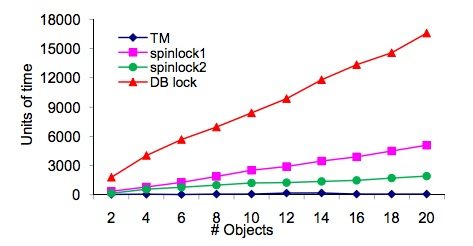
\includegraphics[width=0.3\textwidth]{figure/overhead.jpg}
  \caption{Overhead of CC approaches.}
  \label{fig:fcommon} 
\end{figure}
\section{Project Plan} \label{sec:intro}

Broadly speaking, we plan to:
\begin{itemize}
\item implement two different TSX-based concurrency control schemes for a simple key-value store
\item evaluate the performance of that concurrency control scheme under different workloads
\end{itemize}
The goals of the project are as follows:
\begin{itemize}
\item \textbf{75\% goal:} Implement concurrency control for a key-value store with both HLE and RTM, and compare the performance of these two schemes against each other.
\item \textbf{100\% goal:} Additionally, compare the above approaches with traditional pessimistic concurrency control schemes, specifically spin-locks and a basic lock manager. This will demonstrate the advantages of the hardware-based approach for this task, or else show that this task is not one where the hardware-based approach helps.
\item \textbf{125\% goal:} Additionally, implement a software-based (i.e., timestamp-based) OCC scheme and compare it against the above approaches. This will serve as a basic check that it is in fact the hardware that is the cause of any differences in performance, not just the optimistic approach to concurrency.
\end{itemize}

\subsection{Resources Required}
The only resource absolutely necessary for this project is access to a machine with a Haswell processor. Dong has granted us access to a CMU-owned machine.

It would be useful, though not essential, to have access to the existing codebase that has been used by Professor Andersen's lab to run similar HTM experiments in the past. In particular, it would be helpful to have access to the key-value store implementation used in the lab's in-progress study. We are expecting that Dong will be able to give us access to this, as well.

\subsection{Experiments}
Our experiments are inspired by those reported in \citep{tm-eval-paper}. We will restrict ourselves to a small, fixed number of key-value store entries. In each experiment, we will measure the time it takes to run a randomly generated workload of datastore operations, given a particular CC scheme. Each workload will simply consist of looking up some set of keys and trivially modifying their values (e.g., incrementing). Specifically, we will run the following experiments for each type of CC mechanism:
\begin{enumerate}
\item With several fixed sizes for read/write sets and numbers of threads, vary the contention level between operations on different threads. This will allow us to determine how each of the CC mechanisms scales with respect to contention.
\item With several different fixed contention levels and numbers of threads, vary the size of the read/write sets. This will allow us to determine how each of the CC mechanisms scales with respect to the read/write set. (For HTM, this may be a very important factor, since transactions abort based on conflicts anywhere in the read/write set.)
\item With several different fixed contention levels and read/write set sizes, vary the number of threads running. This will allow us to determine how much benefit each mechanism is able to benefit from adding more parallelism.
\end{enumerate}

\subsection{Work Plan}
The required steps for executing this project are as follows:
\begin{enumerate}
\item Familiarize ourselves with an existing basic key-value store system, such as that built by Professor Andersen's group, or (if that turns out to be impractical) implement our own. If we end up choosing the latter approach, we can minimize implementation effort by keeping the data structures very simple -- just 1-2 hash tables, one for the data and one for locks or to group data entries larger than a cache line (if applicable).
\item Design the structure of the transaction manager to support multiple CC mechanisms.
\item Using the Haswell TSX APIs, implement a transaction manager that optimistically attempts to execute a transaction, and retries according to either an HLE strategy or a custom RTM-specified strategy.
\item Write a system to generate test workloads with different amounts of contention. It should also allow specifying thread assignments if necessary.
\item Run the experiments for the two HTM approaches. Some tweaking will be necessary to find the most informative thread numbers, read/write set sizes, and contention levels.
\item Implement spin-locks and a lock manager.
\item Rerun the experiments for the pessimistic concurrency control approaches.
\item Implement software-based OCC.
\item Rerun the experiments for OCC.
\item Collate/visualize data and write up report.
\end{enumerate}

All of us will work together on items 1 and 2. Two of us (jdunietz and jarulraj) will collaborate (via pair programming) to implement the TSX-based transaction manager. In parallel, twmarsha will implement the workload generator using an agreed-upon interface. jarulraj and twmarsha will each run preliminary versions of one experiment for item 5, and jdunietz will use their results to run the final experiments and collate/visualize the data. twmarsha will implement a lock manager, jarulraj will implement spin-locks, and jdunietz will implement OCC.

\bibliographystyle{plain}
\bibliography{ref}

\end{document}
% end doc
